{\fontsize{12}{14}\selectfont 

\begin{figure}[H]
  \centering
  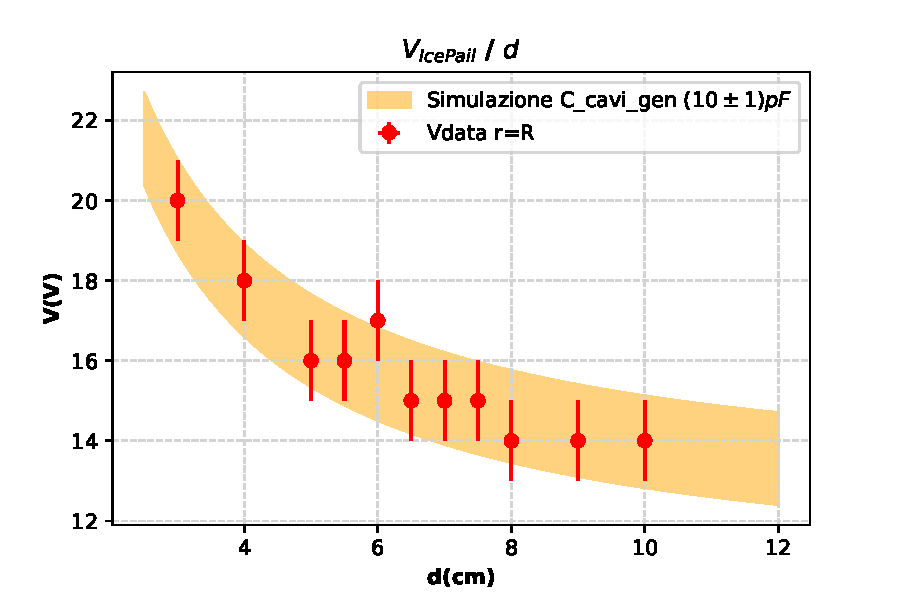
\includegraphics[width=14cm]{Figures/Grafico_Parte3.pdf}
  \caption{Grafico della tensione (in Volt) in funzione della distanza tra le piastre (in centimetri). L'errore sulla tensione è pari a $1.3V$. L'errore sulla distanza è di $1 mm$. La simulazione è stata fatta supponendo una capacità dei cavi che collegano il condensatore al generatore di $(10 \pm 1)pF$, supposizione necessaria ai fini del risultato della simulazione per poter ricreare l'andamento atteso.}
  \label{fig:GraficoParteIII}
\end{figure}


\par}